\section{Partes interesadas}
\sloppy

\subsection{Identificaci\'on y caracterizaci\'on}
Se identifican las partes interesadas como Roles, no como personas, seg\'un lo exigido por ISO/IEC/IEEE 29148:2018 \cite{iso29148} y los fundamentos de ingenier\'ia de requisitos \cite{pohl2025}. La tabla~\ref{tab:stakeholders} registra diez roles, su inter\'es, su influencia, su disponibilidad estimada y la estrategia de participaci\'on propuesta. Los c\'odigos sustituyen a los nombres para evitar la publicaci\'on de datos personales, conforme a la LOPDP \cite{lopdp2021}. La disponibilidad es una estimaci\'on de planificaci\'on, no un dato confirmado por la organizaci\'on.

\begin{table}[htbp]
\centering
\footnotesize
\begin{tabularx}{\linewidth}{|l|p{1.9cm}|Y|p{1.8cm}|p{2.4cm}|X|}
\hline
\thdr{C\'odigo} & \thdr{Rol} & \thdr{Inter\'es principal} & \thdr{Influencia} & \thdr{Disponibilidad} & \thdr{Estrategia de participaci\'on}\\
\hline
AD-01 & Propietario / administrador & Viabilidad econ\'omica y control de la operaci\'on & Alta & Baja & Entrevista individual y validaci\'on final; res\'umenes breves por correo institucional.\\
\hline
GO-01 & Gerente de operaciones & Flujos de sala y cocina sin interrupciones & Alta & Media & Taller de modelado de flujos y revisi\'on de prioridades.\\
\hline
COC-01 & Jefe de cocina & Ordenes claras y tiempos de preparaci\'on & Media & Media & Observaci\'on en turno y entrevista corta posterior.\\
\hline
COC-02 & Personal de cocina & Evitar reprocesos y confusiones & Baja & Media & Observaci\'on an\'onima y preguntas abiertas en el taller.\\
\hline
MES-01 & Mesero/a & Registrar pedidos con rapidez & Baja & Alta & Observaci\'on en sala y cuestionario breve.\\
\hline
CAJ-01 & Cajero/a & Cierre de caja exacto y res\'umenes claros & Media & Media & Entrevista focalizada sobre reglas de cierre.\\
\hline
INV-01 & Encargado de inventario & Existencias suficientes y trazabilidad & Media & Media & Cuestionario estandarizado y revisi\'on de entradas y salidas.\\
\hline
DEL-01 & Repartidor/a & Conocer el estado de cada entrega & Baja & Media & Cuestionario breve de tres preguntas.\\
\hline
CLI-01 & Cliente final & Servicio oportuno y pedido correcto & Baja & Baja & Cuestionario an\'onimo sin datos de identificaci\'on.\\
\hline
PRO-01 & Proveedor local & Reposiciones oportunas & Baja & Alta & Contacto indirecto por medio de INV-01; solo si el responsable lo autoriza.\\
\hline
\end{tabularx}
\caption{Partes interesadas, intereses y estrategia de participaci\'on.}
\label{tab:stakeholders}
\end{table}

\subsection{Matriz poder--inter\'es}
La figura~\ref{fig:matriz} sit\'ua los roles seg\'un su poder de decisi\'on y su inter\'es en el proyecto. La ubicaci\'on es una propuesta derivada de la caracterizaci\'on anterior y se revisar\'a con AD-01 en la sesi\'on de validaci\'on.

\begin{figure}[htbp]
\centering
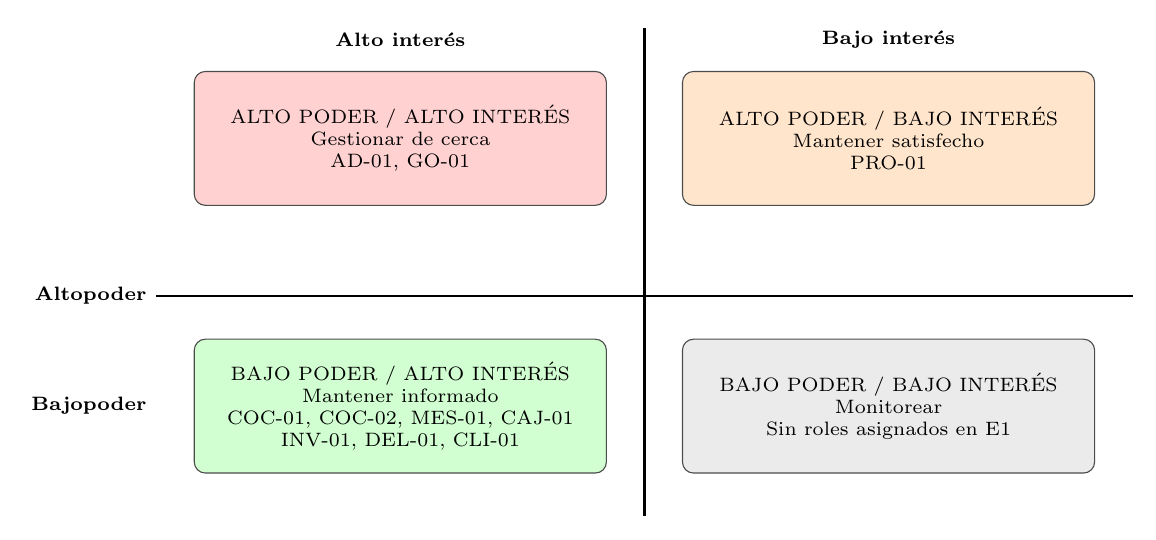
\includegraphics[width=0.88\linewidth]{figuras/poder_interes.png}
\caption{Matriz poder--inter\'es propuesta para El Balcón Restaurant.}
\label{fig:matriz}
\end{figure}

\subsection{Estrategia de participaci\'on por cuadrante}
\begin{itemize}[leftmargin=18pt,itemsep=3pt]
    \item \textbf{Alto poder y alto inter\'es (AD-01, GO-01):} gestionar de cerca. Se les entrevista al inicio y se les presenta el resultado de cada sesi\'on para obtener decisiones y correcciones.
    \item \textbf{Alto poder y bajo inter\'es (PRO-01):} mantener satisfecho. Se le informa solo sobre lo que afecta reposiciones, sin solicitar datos sensibles.
    \item \textbf{Bajo poder y alto inter\'es (COC-01, COC-02, MES-01, CAJ-01, INV-01, DEL-01, CLI-01):} mantener informado. Se les aplica la t\'ecnica que corresponda y se les devuelve un resumen an\'onimo de lo aportado.
    \item \textbf{Bajo poder y bajo inter\'es:} monitorear. No se han asignado roles a este cuadrante en la entrega 1.
\end{itemize}

La estrategia anterior guarda coherencia con las t\'ecnicas planificadas en la secci\'on~7 y con los instrumentos de los ap\'endices: a cada rol se le aplica solo la t\'ecnica que puede responder al tipo de conocimiento que posee \cite{ireb2026}.
